\documentclass[12pt, a4paper]{article}

% ~~~~~~~~~~ Preamble: Packages and Document Setup ~~~~~~~~~~
\usepackage[utf8]{inputenc}
\usepackage{graphicx}
\usepackage{amsmath}
\usepackage{geometry}
\usepackage{setspace}
\usepackage{booktabs} % For better table rules
\usepackage{caption}
\usepackage{subcaption} % For arranging figures
\usepackage{xcolor}     % For colors in tables and text
\usepackage{listings} % For code blocks
\usepackage{hyperref}
\usepackage[style=numeric, sorting=none, backend=biber]{biblatex}
\addbibresource{references.bib} % The .bib file you will create

% Page geometry
\geometry{
 a4paper,
 left=25mm,
 right=25mm,
 top=25mm,
 bottom=25mm,
}

% Hyperlink setup
\hypersetup{
    colorlinks=true,
    linkcolor=blue,
    citecolor=green,
    filecolor=magenta,      
    urlcolor=cyan,
    pdftitle={SPEI Computation and Visualization Pipeline},
    pdfpagemode=FullScreen,
}

% Spacing
\onehalfspacing

% ~~~~~~~~~~ Title and Author ~~~~~~~~~~
\title{\huge\textbf{SPEI Computation and Visualization Pipeline}}
\author{\large Pushkin Mangla \\ \large Department of Computer Science and Engineering, IIT Delhi}
\date{}

% ~~~~~~~~~~ Document Begins ~~~~~~~~~~
\begin{document}

\maketitle
\tableofcontents
\newpage

\begin{abstract}
    \noindent This document presents a complete pipeline for calculating and visualizing the \textbf{SPEI (Standardized Precipitation Evapotranspiration Index)}, a critical tool for drought assessment. The methodology is built upon open-access geospatial datasets, including precipitation (\textbf{P}) data from \textbf{CHIRPS} and Potential Evapotranspiration (\textbf{PET}) data from \textbf{MODIS}. This work is contextualized within broader efforts to build digital public goods for climate resilience, such as the CORE Stack initiative \cite{seth2024core}.
    \newline\newline
    As a case study, this documentation details an analysis for the state of Madhya Pradesh, India, for the years 2004-2023. The primary objective is to assess drought conditions at monthly, seasonal, and annual scales using \textbf{SPEI-1}, \textbf{SPEI-3}, and \textbf{SPEI-12}, respectively.
\end{abstract}

\section{Data Sources}

\begin{table}[h!]
    \centering
    \caption{Primary datasets used for SPEI calculation.}
    \begin{tabular}{p{6cm} p{6cm}}
        \toprule
        \textbf{Dataset Description} & \textbf{Link} \\
        \midrule
        \textbf{CHIRPS Daily v2.0} \newline Precipitation data ($0.05^{\circ}$ resolution), 1981-present & \href{https://developers.google.com/earth-engine/datasets/catalog/UCSB-CHG_CHIRPS_DAILY}{CHIRPS - Earth Engine} \\
        \addlinespace
        \textbf{MODIS MOD16A2GF v6.1} \newline 8-day Potential Evapotranspiration (PET) from MODIS & \href{https://developers.google.com/earth-engine/datasets/catalog/MODIS_061_MOD16A2GF}{MODIS PET - Earth Engine} \\
        \addlinespace
        \textbf{FAO GAUL} \cite{fao2015gaul} \newline Administrative boundaries of Indian states & \href{https://developers.google.com/earth-engine/datasets/catalog/FAO_GAUL_2015_level1}{FAO/GAUL/2015 - Earth Engine} \\
        \bottomrule
    \end{tabular}
\end{table}

\section{Study Area}
The area of interest is \textbf{Madhya Pradesh}, extracted using the FAO/GAUL boundaries dataset \cite{fao2015gaul} by filtering for ADM0\_NAME = India and ADM1\_NAME = Madhya Pradesh. All analysis and exports are spatially clipped to this region.

\section{Methodology}
The pipeline is divided into three main stages: data preparation in Google Earth Engine (GEE), core statistical processing in R, and final visualization in GEE.

\subsection{Step 1: Computation of Monthly P - PET}
The foundation of the SPEI is the climatic water balance ($D$), calculated as the difference between Precipitation (P) and Potential Evapotranspiration (PET). For each month $i$ from January 2004 to December 2023, the water balance for each pixel was calculated as:
\[ D_i = P_i - PET_i \]
This was performed in Google Earth Engine using the following process:
\begin{itemize}
    \item CHIRPS daily data was aggregated into monthly sums to derive total monthly Precipitation ($P_i$).
    \item MODIS PET, provided as 8-day composites, was also aggregated into monthly sums and rescaled by a factor of 0.1 to derive total monthly Potential Evapotranspiration ($PET_i$).
    \item The monthly difference ($D_i$) was computed and exported as 240 individual GeoTIFF files, one for each month in the study period.
\end{itemize}
The GEE script for this export is available externally.
\begin{center}
    \textit{The GEE script can be found at: \href{https://github.com/Actuallyanonymous/spei-drought-analysis-pipeline/blob/main/scripts/01_gee_export_pp-et.py}{01\_gee\_export\_pp-et.py}}
\end{center}

\subsection{Step 2: SPEI Standardization in R}
The core of the SPEI calculation was performed in the R programming language, following the exact methodology of the IIT Gandhinagar paper \cite{mishra2023spei} to ensure scientific rigor and consistency. We utilized the official \textbf{`SPEI` package} for R, which is the global standard for this analysis and is used by resources such as the SPEI Global Drought Monitor \cite{spei_csic}.

The standardization process transforms the raw, location-specific water balance data ($D_i$) into a universal, comparable index. This is a multi-step statistical process.

\subsubsection{Aggregation at Different Timescales}
Drought is a multi-scalar phenomenon. To capture this, the water balance data is first aggregated at different timescales by calculating a rolling sum. The aggregated series $D^k$ for a given month $n$ and timescale $k$ is:
\[ D^k_n = \sum_{i=0}^{k-1} D_{n-i}, \quad k \in \{1, 3, 12\} \]
\begin{itemize}
    \item \textbf{SPEI-1 (k=1):} Reflects short-term monthly conditions, relevant for agricultural drought.
    \item \textbf{SPEI-3 (k=3):} Reflects medium-term seasonal conditions, relevant for hydrological drought.
    \item \textbf{SPEI-12 (k=12):} Reflects long-term annual conditions, relevant for water supply and major droughts.
\end{itemize}

\subsubsection{Fitting a Probability Distribution}
The aggregated water balance data ($D^k$) does not follow a normal (Gaussian) distribution; it is often skewed. Therefore, the simple Z-score formula (`(value-mean)/std\_dev`) cannot be used. Instead, a more flexible, three-parameter \textbf{Log-Logistic} probability distribution is fitted to the time series of the aggregated data, as validated by numerous studies \cite{vicente2010multiscalar, stagge2015candidate}. The Cumulative Distribution Function (CDF) for this distribution is given by:
\[ F(x) = \left[1 + \left(\frac{\alpha}{x-\gamma}\right)^\beta\right]^{-1} \]
where $\alpha$, $\beta$, and $\gamma$ are the scale, shape, and origin parameters, respectively, which are estimated from the data.

\subsubsection{Parameter Estimation via the Method of L-moments}
To find the optimal parameters ($\alpha, \beta, \gamma$) for the Log-Logistic curve, the `SPEI` package uses the **Method of L-moments**. This technique is statistically more robust than conventional moments (mean, variance, skewness) because it is calculated from linear combinations of the ordered data, making it far less sensitive to outliers. The process is as follows:
\begin{enumerate}
    \item The first three sample L-moments are calculated from the raw P-PET data series:
    \begin{itemize}
        \item $\lambda_1$: A measure of location (L-location).
        \item $\lambda_2$: A measure of scale (L-scale).
        \item $\tau_3$: A measure of skewness (L-skewness ratio).
    \end{itemize}
    \item The `SPEI` package then uses established mathematical formulas to directly derive the values of $\alpha$, $\beta$, and $\gamma$ from these calculated L-moments. This provides a robust fit that correctly handles the negative values present in the P-PET data.
\end{enumerate}

\subsubsection{Final Standardization to a Z-score}
The final step is to convert the fitted probability into a universal index.
\begin{enumerate}
    \item The CDF of the fitted Log-Logistic curve, $F(x)$, is used to find the cumulative probability $P$ of a given water balance value.
    \item This probability $P$ is then transformed into a standard normal variable (a Z-score) using the inverse of the standard normal CDF, also known as the quantile function ($\Phi^{-1}$). This function asks, "On a perfect bell curve, what Z-score corresponds to this probability/percentile?"
    \[ \text{SPEI} = \Phi^{-1}(P) \]
    This final Z-score is the SPEI value, where a value of 0 is perfectly average, negative values indicate drought, and positive values indicate wetness.
\end{enumerate}

\subsubsection{Implementation Process}
The R script automates this entire process. It loads the 240 P-PET images into a raster brick and uses a robust, block-processing method to apply a function to each pixel. This function converts the pixel's 20-year history into a time series and uses the `spei()` function to perform the entire calculation (L-moment fitting, CDF calculation, and standardization) for SPEI-1, SPEI-3, and SPEI-12. The script then saves the results as properly georeferenced GeoTIFF files.
\begin{center}
    \textit{The full R script can be found at: \href{https://github.com/Actuallyanonymous/spei-drought-analysis-pipeline/blob/main/scripts/02_calculate_spei.R}{02\_calculate\_spei.R}}
\end{center}

\subsection{Step 3: Visualization in Google Earth Engine}
Selected SPEI images were uploaded as assets to Google Earth Engine for visualization and validation.
\begin{center}
    \textit{The full GEE script can be found at: \href{https://github.com/Actuallyanonymous/spei-drought-analysis-pipeline/blob/main/scripts/03_gee_visualize_spei.js}{03\_gee\_visualize\_spei.js}}
\end{center}

\subsection{Result Verification Example}
The multi-scalar nature of SPEI allows for a comprehensive analysis of drought events. The year \textbf{2015} serves as an excellent case study. The SPEI-1 for June 2015 (Figure \ref{fig:2015_results}a) indicates significant drought conditions at the beginning of the year.

However, the SPEI-3 for the monsoon season of July-September (Figure \ref{fig:2015_results}b) shows a period of near-normal or even slightly wet conditions. This can be attributed to monsoon rainfall temporarily alleviating the water deficit.

Despite the mid-year relief, the SPEI-12 for the entire calendar year (Figure \ref{fig:2015_results}c) reveals a severe to extreme drought, confirming that the annual water balance was overwhelmingly negative. This aligns with ground reports from news articles \cite{sandrp2015} and government reports \cite{dpd2015}. This demonstrates the pipeline's ability to capture both short-term variations and the overarching annual drought severity.

\begin{figure}[h!]
    \centering
    \begin{subfigure}[b]{0.48\textwidth}
        \centering
        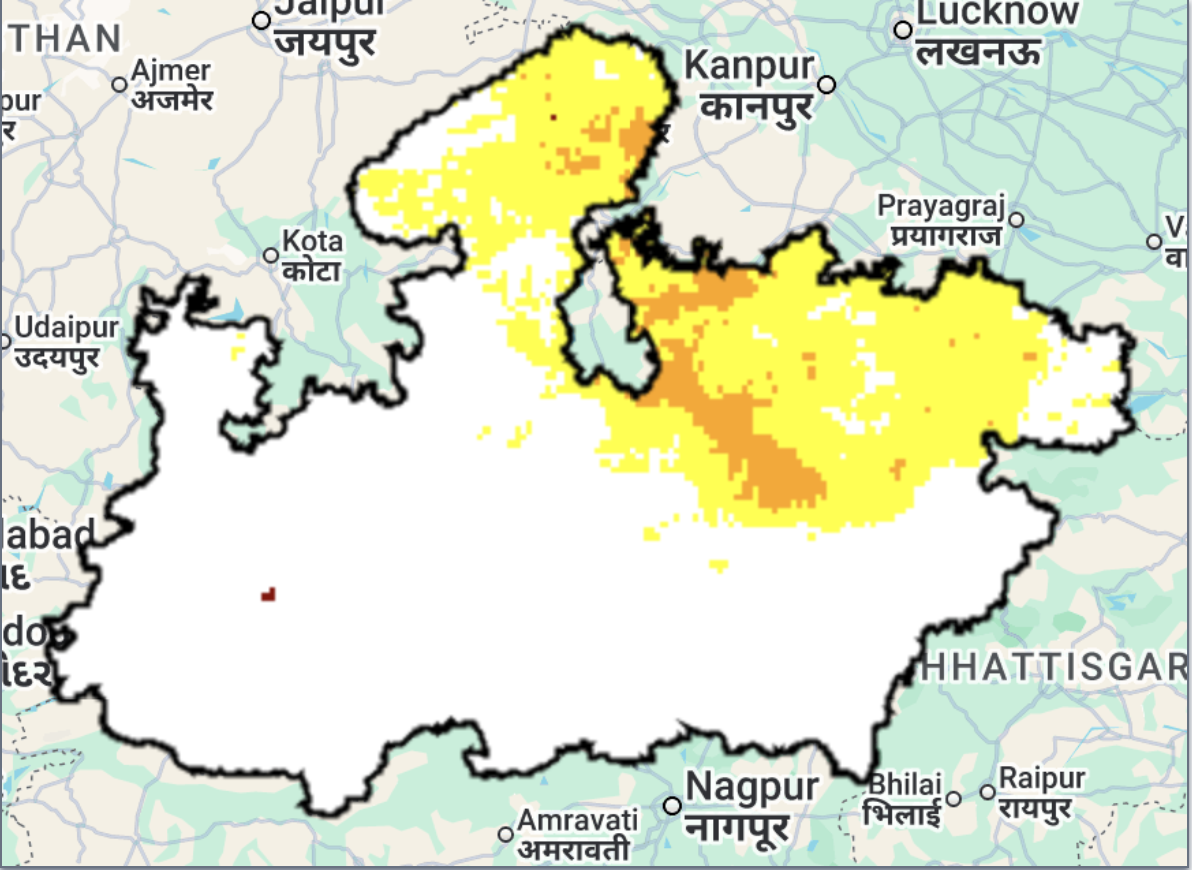
\includegraphics[width=\textwidth]{spei_june_2015.png}
        \caption{SPEI-1 for June 2015, showing initial drought conditions.}
        \label{fig:2015_jan}
    \end{subfigure}
    \hfill
    \begin{subfigure}[b]{0.48\textwidth}
        \centering
        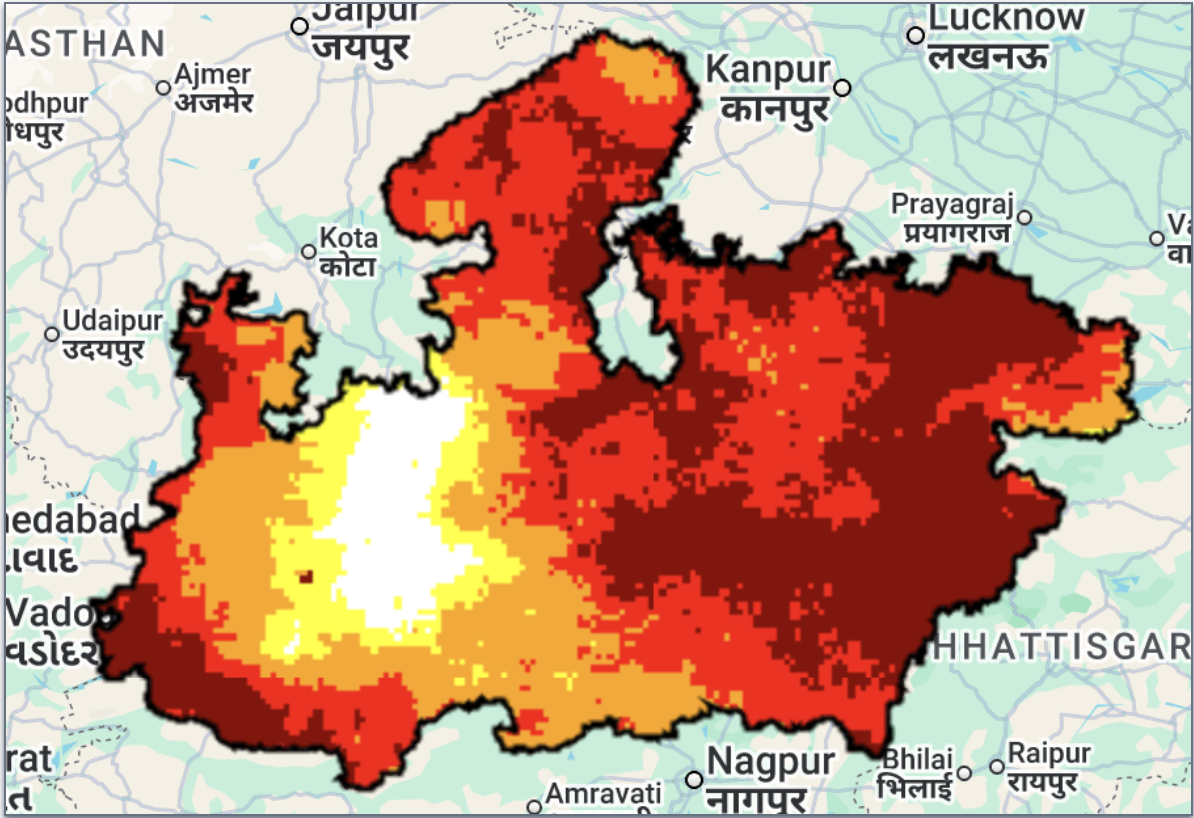
\includegraphics[width=\textwidth]{spei_jul-sep_2015.png}
        \caption{SPEI-3 for July-September 2015, showing temporary relief.}
        \label{fig:2015_season3}
    \end{subfigure}
    
    \vspace{1cm} % Add some vertical space
    
    \begin{subfigure}[b]{0.6\textwidth}
        \centering
        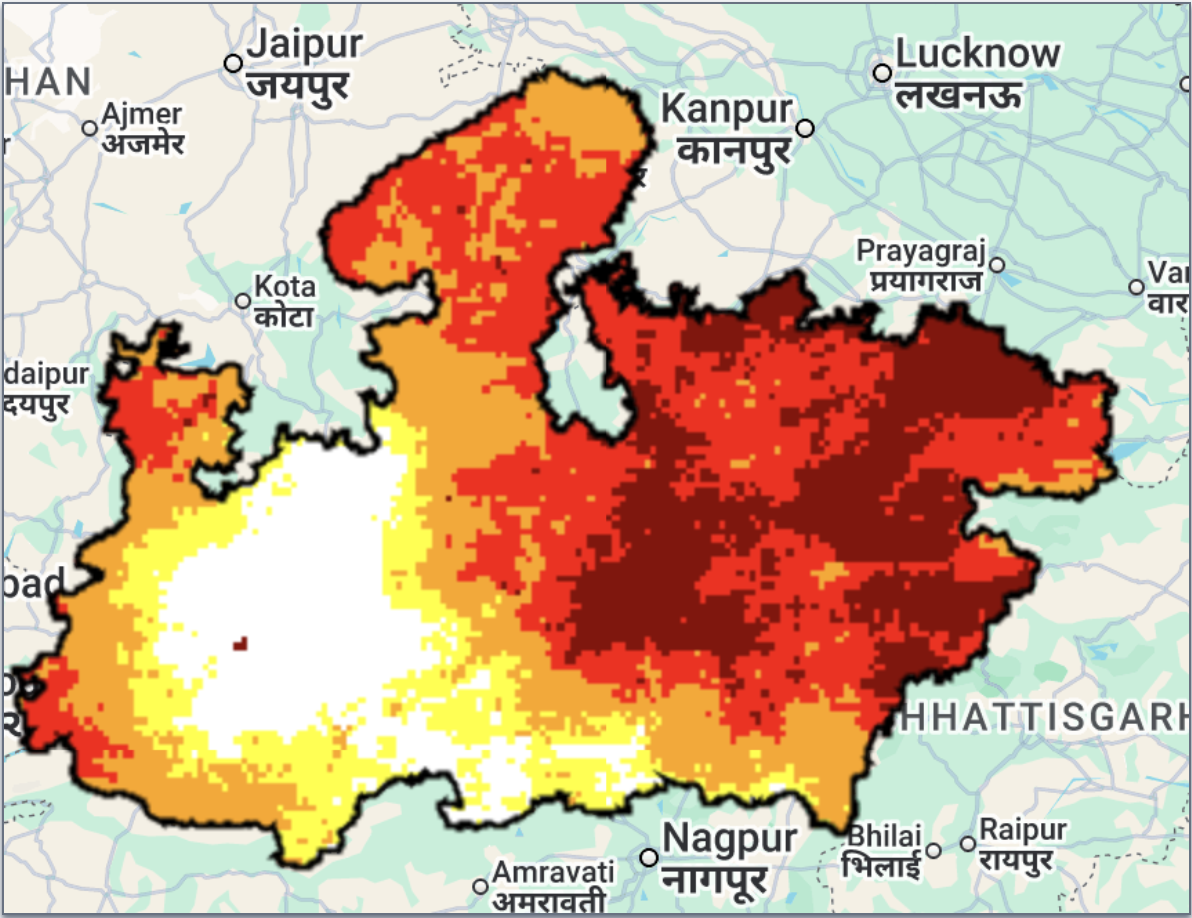
\includegraphics[width=\textwidth]{spei_annual_2015.png}
        \caption{SPEI-12 for the full year 2015, confirming severe annual drought.}
        \label{fig:2015_annual}
    \end{subfigure}
    \caption{Multi-scalar SPEI analysis for the 2015 drought event in Madhya Pradesh.}
    \label{fig:2015_results}
\end{figure}

\clearpage % This command ensures all figures are placed before the next section

\section{References}
\printbibliography

\vspace{1cm}
\noindent \textbf{NOTE:} The SPEI-12 here is measured for the calendar year. This can be changed to an
agricultural year as per requirements.

\newpage

\noindent This pipeline was developed and implemented by: \\
\textbf{Pushkin Mangla} \\
B.Tech.-M.Tech. Dual Degree Student \\
Department of Computer Science and Engineering, Class of 2029 \\
Indian Institute of Technology Delhi

\vspace{1cm}

\noindent Under the academic supervision of: \\
\textbf{Prof. Aaditeshwar Seth} \\
Department of Computer Science and Engineering \\
Indian Institute of Technology Delhi

\end{document}
